% Made up for the tikra benchmark.
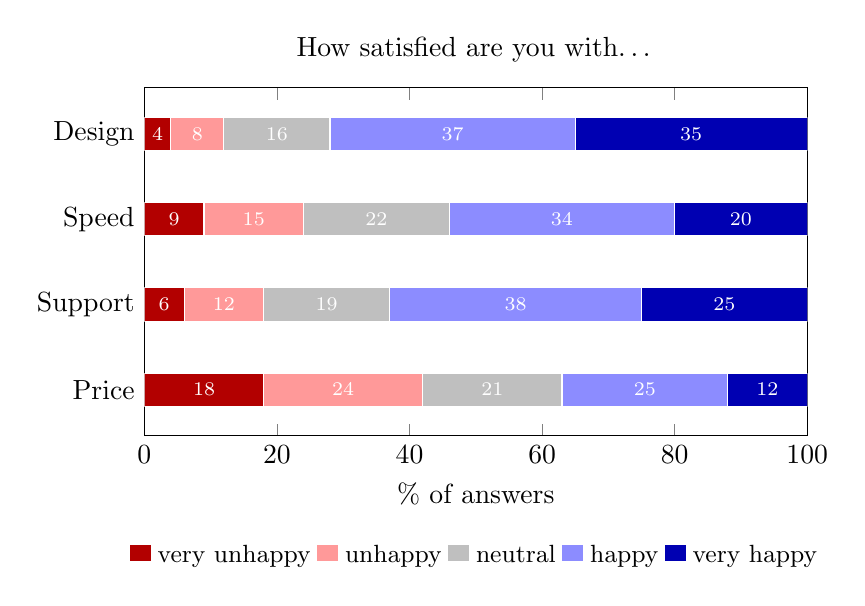
\begin{tikzpicture}
\begin{axis}[xbar stacked, bar width=12pt, width=10cm, height=6cm, xmin=0, xmax=100,
    symbolic y coords={Price, Support, Speed, Design}, ytick=data, xlabel={\% of answers},
    title={How satisfied are you with\dots}, enlarge y limits=0.18,
    legend style={at={(0.5,-0.28)}, anchor=north, legend columns=-1, font=\small, draw=none},
    nodes near coords, every node near coord/.append style={font=\scriptsize, white}]
  \addplot[fill=red!70!black, draw=white] coordinates {(18,Price) (6,Support) (9,Speed) (4,Design)};
  \addplot[fill=red!40, draw=white] coordinates {(24,Price) (12,Support) (15,Speed) (8,Design)};
  \addplot[fill=gray!50, draw=white] coordinates {(21,Price) (19,Support) (22,Speed) (16,Design)};
  \addplot[fill=blue!45, draw=white] coordinates {(25,Price) (38,Support) (34,Speed) (37,Design)};
  \addplot[fill=blue!70!black, draw=white] coordinates {(12,Price) (25,Support) (20,Speed) (35,Design)};
  \legend{very unhappy, unhappy, neutral, happy, very happy}
\end{axis}
\end{tikzpicture}
